\documentclass[12pt]{article}

% \usepackage[default]{sourcecodepro}
% \usepackage[T1]{fontenc}

\usepackage{amsfonts, lipsum}
\usepackage{amsmath,amssymb, amscd,amsbsy, bbm, amsthm, enumerate}
\usepackage{mdframed, titlesec, setspace,verbatim, multicol}
\usepackage[top=1in, bottom=1in, left=.45in, right=.45in]{geometry}
\usepackage[unicode]{hyperref}
\usepackage{tikz, pgfplots, xcolor, fancyhdr}
\usepackage{graphicx, caption, subcaption}
\usepackage{stmaryrd}

\setlength{\parindent}{0pt}
\setlength{\textheight}{9in}

%%% Header and Footer Info
\pagestyle{fancy}
% \fancyhead[L]{{\large CSE431 Assignment 4}}
% \fancyhead[C]{}
% \fancyhead[R]{Name: Bradley Bauer}
\fancyhead[L]{\large CSE 431 Assignment 4 }
\fancyhead[C]{}
\fancyhead[R]{\large Question 2}

\theoremstyle{definition}

%%% These are some shortcuts that are handy
\def\real{{\mathbb R}}
\def\Natural{\mathbb{N}}
\def\dx{\textnormal{dx}}
\def\dy{\textnormal{dy}}
\def\dz{\textnormal{dz}}
\def\dt{\textnormal{dt}}
\def\ds{\textnormal{ds}}
\def\dw{\textnormal{dw}}
\def\Re{\textnormal{Re}}
\def\Im{\textnormal{Im}}
\def\exp{\textnormal{exp}}
\def\interior{\textnormal{interior}}
\def\al{\alpha}
\def\del{\delta}
\def\Del{\Delta}
\def\gam{\gamma}
\def\Gam{\Gamma}
\def\Om{\Omega}
\def\ep{\varepsilon}
\def\lam{\lambda}
\def\rational{{\mathbb Q}}
\def\integer{{\mathbb Z}}
\def\Q{{\mathbb Q}}
\def\Z{{\mathbb Z}}
\def\N{{\mathbb N}}
\def\R{{\mathbb R}}
\def\grad{\nabla}
\def\C{\mathcal C}
\def\P{\mathcal P}
\def\T{\mathcal T}
\def\I{\mathcal I}
\newcommand{\abs}[1]{\left| #1 \right|}
\newcommand{\inner}[1]{\langle #1 \rangle}
\newcommand{\norm}[1]{\left\lVert#1\right\rVert}
\newcommand{\spanvect}{\textnormal{span}}
\newcommand{\union}{\cup}
\newcommand{\Union}{\bigcup}
\def\intersect{\cap}
\def\Intersect{\bigcap}

\newtheorem{innercustomthm}{}
\newenvironment{question}[1]
  {\renewcommand\theinnercustomthm{#1}\innercustomthm}
  {\endinnercustomthm}

\begin{document}

\begin{question}{Hypothesis}
    I expect the optimal value for k to be the same as the cross over value found in problem 1.
\end{question}

\begin{question}{Methods}
    The experiment is ran on Ubuntu 19.04. GCC version is 8.3 and python version is 3.7.3.
    Also, matplotlib and pandas are dependencies of plot.py\\\\
    To run the experiment, first compile
    $$\text{g++ -fconcepts -std=c++2a -O3 code.cpp}$$
    Then execute $$\text{./a.out}$$
    To plot the results use
    $$\text{python3 plot.py}$$
    The code runs hybridsort, quicksort, and insertion sort on vectors of uniform random integers (from [0,2**31-1]) of length n=1,...,700.
    For each input size n we run the algorithms for each value of k=1,...,200 where k is the quicksort/insertionsort cross over parameter in hybridsort.
\end{question}
\newpage
\begin{question}{Results}
$\\$
\vspace{-1cm}
\begin{figure}[h]
  \centering
  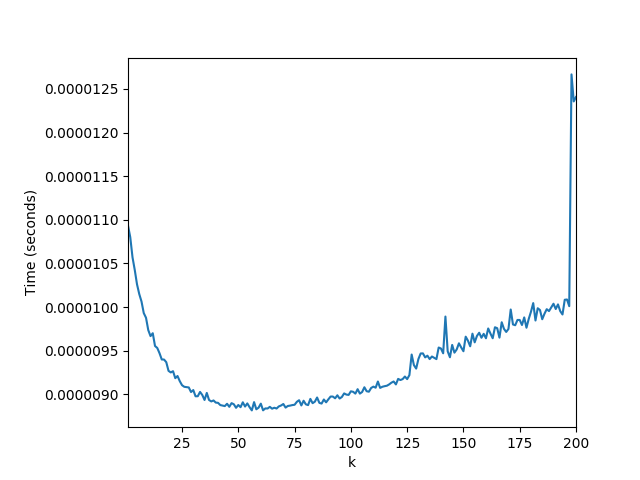
\includegraphics[width=\textwidth]{Figure1.png}
  \caption{}
  \label{fig:boat1}
\end{figure}

\begin{figure}[h]
  \centering
  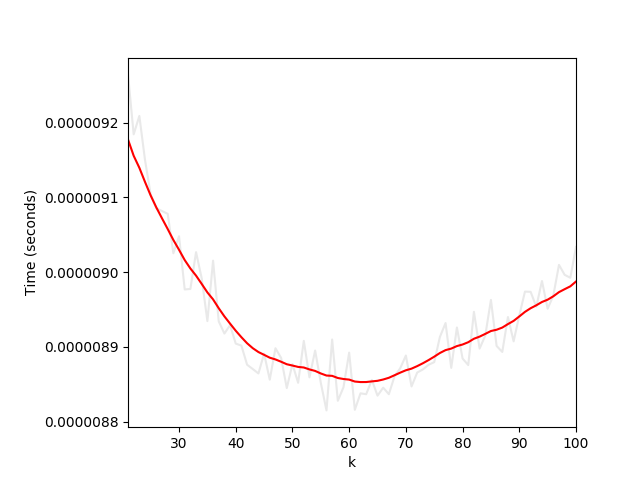
\includegraphics[width=\textwidth]{Figure2.png}
  \caption{}
  \label{fig:boat2}
\end{figure}

\begin{figure}[h]
  \centering
  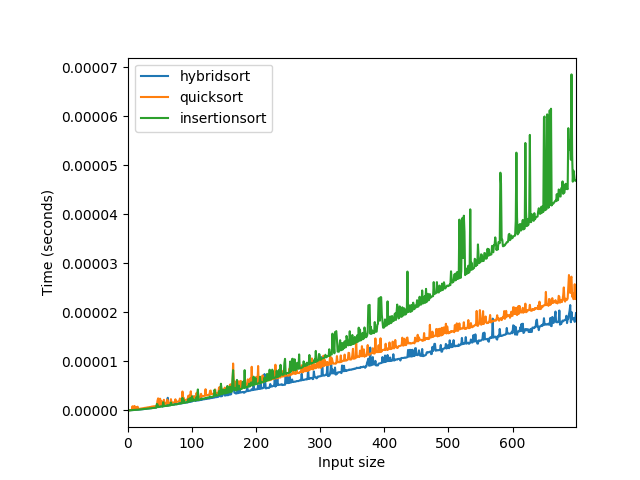
\includegraphics[width=\textwidth]{Figure3.png}
  \caption{}
  \label{fig:boat3}
\end{figure}
%\begin{figure}[h]

Figure 1 shows a plot of the average performance (vertical axis, averaged across n=1,...,700) of hybridsort for a given k value (horizontal axis).
\newpage
Figure 2 is a zoomed in and smoothed plot of the same data as in Figure 1.
\newpage
Figure 3 compares hybridsort, with the optimal k parameter, against insertionsort and quicksort for input sizes n=1,...700.

\end{question}

\begin{question}{Discussion}
    Figure 2 shows that the optimal k value for hybridsort is roughly 61.
    This is not the same as the insertionsort/quicksort cross over point found in question 1.
    If k is equal to the value found in question 1 then the time taken by insertionsort is equal to the time taken by quicksort on partitions of size k.
    This is not optimal since then we have no performance gain when switching to insertionsort.
    So the optimal k value should be less than the cross over value found in question 1, which is what we observe (since the value in question 1 was around 180).
    \\
    Let $TQ_n$ be the time taken by quicksort on inputs of size n and let $TI_n$ to be the time taken by insertion sort on inputs of size n.
    Then my new hypothesis is that an optimal k should maximize
    $$\frac{n}{k}(TQ_k - TI_k)  =(\text{num partitions})*(\text{time gained by using insertion sort})$$
    I think there is a more advanced analysis using a tree to describe work done by hybridsort.
    Then we would want to choose $k$ to minimize the sum $a+b$ where $a$=work done by quicksort above level $\log{\frac{n}{k}}$ and $b$=work done by insertion sort on $\frac{n}{k}$ partitions each of size $k$.
    Maybe something like this : $c_0n\log{\frac{n}{k}}+\frac{n}{k}c_1\frac{k(k-1)}{2}$.
    Then plugging in $c_1=.000000000097$, $c_0=.000000003$, and $n=491$ we get the following plot\\
\begin{figure}[h]
  \centering
  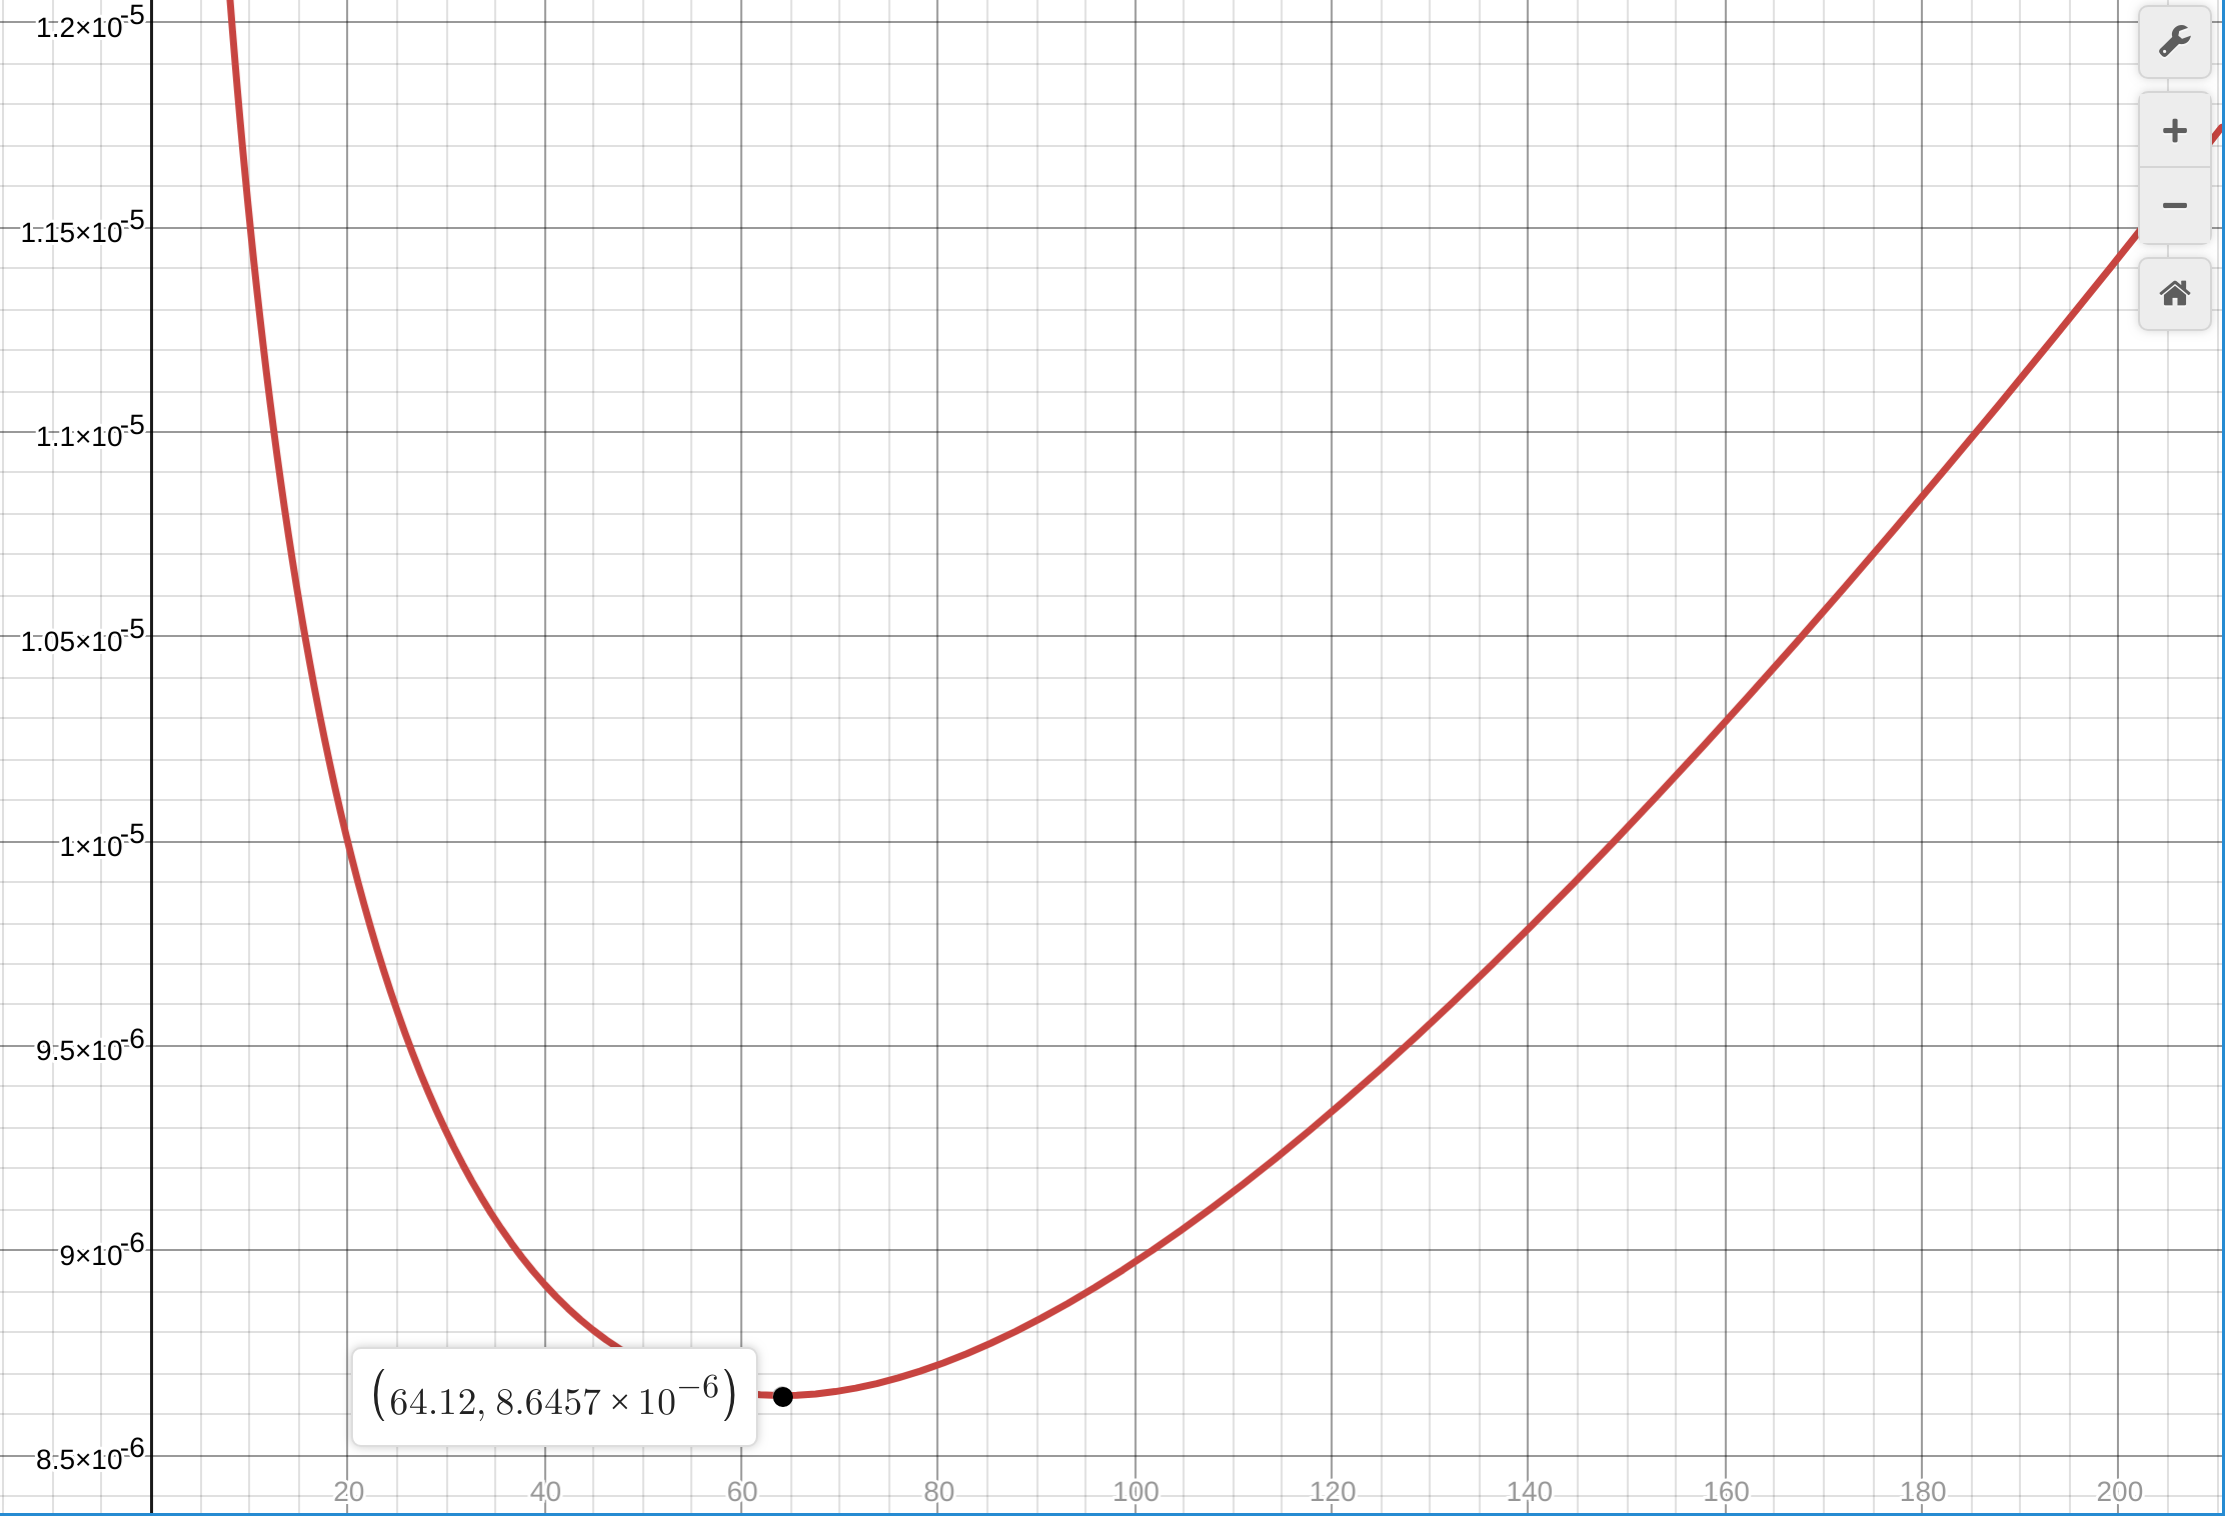
\includegraphics[width=\textwidth]{asdf.png}
  \caption{}
  \label{fig:boat3}
\end{figure}
\\
    $c_1$ was found by fitting a quadratic to the Time(n) function of my insertionsort.
    $c_0$ was a guess.
    But, given these values, the resulting plot looks similar to figure 1 and 2.

\end{question}

\begin{question}{Conclusion}
    Hybridsort with a k value of 61 is faster than quicksort by some constant factor.
\end{question}

\end{document}
